\documentclass[conference]{IEEEtran} 
\IEEEoverridecommandlockouts
\renewcommand{\baselinestretch}{0.985}
\usepackage{graphicx}
\usepackage{booktabs}
\usepackage{amsfonts}
\usepackage{amsmath}
\usepackage{multirow}
\usepackage{makecell}
\usepackage[colorlinks=true, allcolors=blue]{hyperref}
\usepackage{subcaption}

\def\BibTeX{{\rm B\kern-.05em{\sc i\kern-.025em b}\kern-.08em
    T\kern-.1667em\lower.7ex\hbox{E}\kern-.125emX}}

\graphicspath{ {.} }
\let\vec\mathbf
\DeclareMathOperator*{\argmin}{arg\,min}

\newcommand{\etal}{\textit{et al}.}

\title{Semi-Supervised Medical Imaging Segmentation Using DatasetGAN}


\author{\IEEEauthorblockN{Zong Fan}
\IEEEauthorblockA{\textit{Dept. Bioengineering}, UIUC \\
zongfan2@illinois.edu}
}

\begin{document}
\maketitle

\vspace{-0.5cm}
\begin{abstract}
\maketitle

\end{abstract}
Semantic segmentation is an important research field in medical imaging analysis, which is widely used for diagnosis and treatment plans. However, medical segmentation usually requires domain experts to manually draw the contours accurately, making the annotation process slow and laborious. It's very difficult to obtain a large enough dataset for training segmentation networks in many clinical applications.  
Semi-supervised learning (SSL) methods are proposed to reduce the need for a large annotated dataset. However, the widely-used methods including pseudo-labeling and consistency regularization pose challenges in choosing the labeling seeds and perturbation strategy. 
In addition, few previous SSL studies are focused on segmentation tasks. GAN-based SSL is promising since GAN is capable of learning the distribution of unlabeled data and recent DatasetGAN shows the potential of latent representations of GAN in predicting segmentation data. 
Therefore, in this study, we utilize the idea of DatasetGAN and modify it to adapt to a small-scale medical imaging dataset. 
By replacing the original StyleGAN generator with StyleGAN2 generator and introducing the adaptive discriminator augmentation strategy during the training of the style-based generator, the generated image quality keeps relatively high even on small dataset. 
A set of experiments were employed to validate our modifications. Also, various factors that might affect the generation quality were investigated.
A well-trained model could function as a segmentation labeling factory to automatically produce massive datasets containing high-quality image-segmented mask pairs. 
It indicates the potential of applying the synthetic dataset as an objective evaluator of segmentation networks.

% \vspace{-0.3cm}
\section{Introduction}

\label{sec:intro}

Deep learning is playing an important role in various medical imaging applications, ranging from disease diagnosis~\cite{Yadav2019DeepCN} to lesion segmentation~\cite{shorten2019survey}. 
Particularly, pixel-wise segmentation is one of the major fundamental research challenges. 
Segmentation of particular organs or lesions in the medical images is the prerequisite for further diagnostic applications like disease classification, staging and grading. 
However, training deep neural networks (DNNs) usually needs large amounts of labeled data to achieve satisfying model performance~\cite{shorten2019survey}, while fine-grained segmentation annotation is a really expensive, time-consuming and laborious task, especially medical images usually need skilled experts to accurately depict the region of interests. 
This drawback limits the availability of a large segmentation dataset for most clinical problems. The unavailability of large annotated dataset makes it impractical to train a satisfying segmentation network via the fully-supervised learning strategy. 
In addition, it's not easy to generalize a trained model outside the training dataset, especially when the images are captured via different sensors~\cite{Aggarwal2021DiagnosticAO}. 
That means the time-consuming re-labeling of the dataset across different imaging sensors is required to tune the model~\cite{zhuang2020comprehensive}. 

To solve this problem, many techniques have been proposed to lower the requirement for annotated data. Semi-supervised learning (SSL) is one of the most popular approaches which construct models with both labeled and unlabeled data. They could be roughly categorized into 4 categories: pseudo-labeling, consistency regularization, generative methods, and graph-based methods~\cite{Yang2021ASO}. The most commonly-used methods are pseudo-labeling and consistency regularization. Pseudo-labeling mainly employs iterative training and prediction strategy to predict pseudo-labels of unannotated data and expand the labeled dataset for the next iteration~\cite{Yang2021ASO}. Consistency regularization is based on the assumption that extra perturbation imposed on the input data should not change the output of the model~\cite{Yang2021ASO}. Consistency loss terms are introduced to find a smooth manifold of the dataset to regularize the predictions for both labeled and unlabeled samples. However, the former method usually needs representative initial labeled data, posing a strict requirement in understanding the dataset distribution. Also, the later method faces another difficult challenge: how to choose a proper unlabeled data perturbation for the dataset. 

Another popular approach is to leverage the generative adversarial network (GAN)~\cite{Goodfellow2014GenerativeAN} for facilitating SSL, because GAN could learn the distribution of real data from the unlabeled samples. GANs are usually utilized via re-using features from the discriminator, using GAN-generated data to regularize a classifier, using synthesized samples as additional training data~\cite{Yang2021ASO}. However, previous studies mainly employed GAN for classification tasks, with little achievement on segmentation tasks.
Recently, several studies have extended generative adversarial networks into low-budget image segmentation annotating factories, which could synthesize pairs of realistic images and corresponding segmentation masks without much annotation work~\cite{Zhang2021DatasetGANEL,Li2021SemanticSW}. 
These methods are developed based on StyleGAN [3], a modern GAN which could synthesize high-quality high-resolution images due to disentangled representation design, to decode the semantically meaningful intermediated feature maps from the well-trained StyleGAN generator to get the segmentation mask along with the simultaneously generated image. 
Ideally, if these GANs could approximate the target image and annotation domain perfectly, the generated segmented image dataset could be used as the real dataset in training the segmentation network. 
In the original DatasetGAN paper,
they have shown that the well-trained DatasetGAN could synthesize massive datasets of high-quality images and corresponding segmented images using natural images.
Training segmentation networks on the synthesized dataset achieve almost identical performance compared to training on real data. 
However, DatasetGAN has its limitations. First, training a StyleGAN with diverse styles usually requires large amounts of images, which might be impractical for small-scale medical imaging datasets. 
Second, StyleGAN occasionally generates noisy images with artifacts due to its intrinsic network design. 

In this study, we utilize DatasetGAN's idea and modify it to accommodate the task of generating segmentation data automatically on small-scale medical image datasets. 
First, the StyleGAN generator is replaced with StyleGAN2 whose network structure is optimized to alleviate the noise and artifacts. 
Second, the adaptive discriminator augmentation (ADA) technique~\cite{karras2020training} is utilized to improve the performance and suppress overfitting using a small training dataset.  
A set of experiments were conducted on a dataset called SegTHOR~\cite{Lambert2020SegTHORSO} and the results verified the effectiveness of our modification. 
The ablation studies analyzed the factors that probably affected the performance of DatasetGAN, deepening the understanding of the attributes of this framework in practical applications. 
This method holds the potential to be applied to other medical segmentation tasks. 
In addition, the synthetic dataset could be treated as the standard dataset in any field of interest for objective evaluation of segmentation algorithms. 
This helps greatly determine whether certain techniques or modifications really benefit the segmentation performance. 


\section{Methods}

\subsection{Background: DatasetGAN implementation}
As shown in Fig.~\ref{fig:workflow} DatasetGAN-StyleGAN2 is composed of two major components - StyleGAN2 generator and style interpreter. The StyleGAN2 framework is trained on the target medical imaging dataset, to make the generator manipulate the distribution of target images. The trained StyleGAN2 generator produces not only the images but also intermediate latent from the style blocks. 
The style interpreter contains two stages: 1) latent feature map extractor and 2) pixel classifier ensemble. The former stage upsamples and combines all the latents to produce a high-dimensional latent feature map with the same shape as generated image. The later stage predicts the class label of each pixel by the use of its high-dimensional vector on the extracted latent feature map, thus producing the corresponding segmentation map of the generated image. Forward a random vector through the trained DatasetGAN-StyleGAN2 could produce a pair of image and automatically annotated segmented image. 


\begin{figure*}[!ht]
  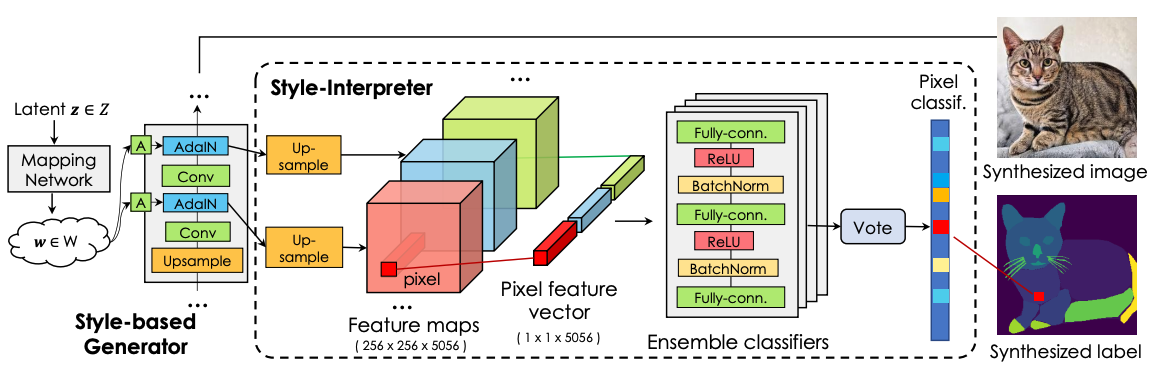
\includegraphics[width=\textwidth]{./fig/datasetgan_framework.png} 
  \caption{The workflow of DatasetGAN to generate target images and corresponding segmentation mask images. Image credit: Zhang \etal, 2021\cite{Zhang2021DatasetGANEL}}
  \label{fig:workflow}
\end{figure*}


\subsubsection{StyleGAN generator for generating medical images}
\label{sec:stylegan}
The StyleGAN~\cite{Karras2019ASG} generator plays the key role in synthesizing high-quality images in the DatasetGAN framework. 
The hypothesis is that a well-trained style-based generator could extract the meaningful semantic information by the progressive style blocks so that the generated fake images are realistic enough to fool the discriminator. 
As shown in Fig.~\ref{fig:stylegan}, the StyleGAN generator contains a mapping network $f$ and a synthesis network $g$. The mapping network contains multiple fully-connected (FC) layers, mapping the latent vector $z\in Z$ drawn from a normal distribution to an intermediate style vector $w\in W$. 
Then the style vector is injected into each style block in the synthesis network via affine transformation. 
The StyleGAN generator has $log_2(m)$ style blocks where $m$ is the training image size and each style block doubles the size of the previous feature map from the previous style block. 
In this study, we set $m=256$ and there are 7 style blocks in a progressive fashion. The StyleGAN2 generator is to synthesize an image $256\times 256$ pixels corresponding to a random latent vector $z$.

\begin{figure}[!ht]
  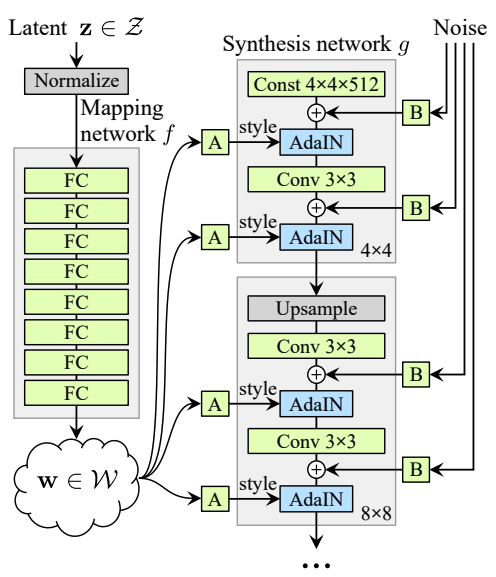
\includegraphics[width=0.5\textwidth]{./fig/stylegan_arch.png} 
  \caption{The architecture of the style-based generator. \fbox{A} denotes a learned affine transform from intermediate latent space $\mathcal{W}$ that produces a style and \fbox{B} is a noise broadcast operation.
  $w$ is the learned weights, $b$ is biases, and $c$ is constant input. Image credit: Karras \etal, 2021\cite{Karras2019ASG}}
  \label{fig:stylegan}
\end{figure}


\subsubsection{Style interpreter for generating segmented images}
\label{sec:interpreter}
The style interpreter consists of two steps: upsample and combine the intermediate latent feature and predict pixel label via pixel classifier ensemble. 

\noindent \textbf{Upsample and combine intermediate features}: 
\label{sec:extactor}
In the DatasetGAN framework, the latent features from the style-based generator are extracted after each AdaIN layer and each style block produces 2 latent features. Up to 14 latent features are extracted in this case, with different sizes of feature resolution and channels. 
All the latent features $\{L_1, L_2, ..., L_14\}$ are upsampled to the largest feature map size, as well as the desired generated image size. 
In our study, these latent features are upsampled to $256\times 256$ pixels. Then the latents are concatenated into a 3D feature map $F$ with shape (256, 256, C), where $C=sum(\# channel\ of\ L_i)$. 
This step is training-free.


\noindent \textbf{Pixel classifier ensemble}:
\label{sec:classifier}
In DatasetGAN, the image segmentation task is treated as a per-pixel classification task. 
As shown in Fig.~\ref{fig:interpreter}, the pixel classifier ensemble is a set of $n$ pixel classifiers with identical network structure. 
The ensemble design aims to reduce the dispersion of predictions and classifier performance, since the style-based generator might inject noise in the synthesized data occasionally~\cite{Karras2020AnalyzingAI}. 
A single pixel classifier $P_i$ predicts the class label of each pixel on top of its M-dimensional pixel vector $F_{i,j}$ on the latent feature map $F$, where $i,j$ is the location indices on $F$. 
Applying the pixel classifier ensemble ${P_1, P_2, ..., P_n}$ to the pixel vector would produce $n$ predicted label ensemble. Then majority voting strategy is employed at testing time to select the most common label as the pixel's class label. 
By iterating all pixels on $F$, the segmented mask image corresponding to the image generated via random latent $z$ is obtained.   

In our study, we set $n=10$ for the pixel classifier ensemble. The network architecture of pixel classifier consists of 3 FC layer interconnected by consequent batch normalization (BN) layer and ReLU activation layer. The 3 FC layers have 2496, 256, 128 neurons, respectively. 
\begin{figure*}[!ht]
  \centering 
  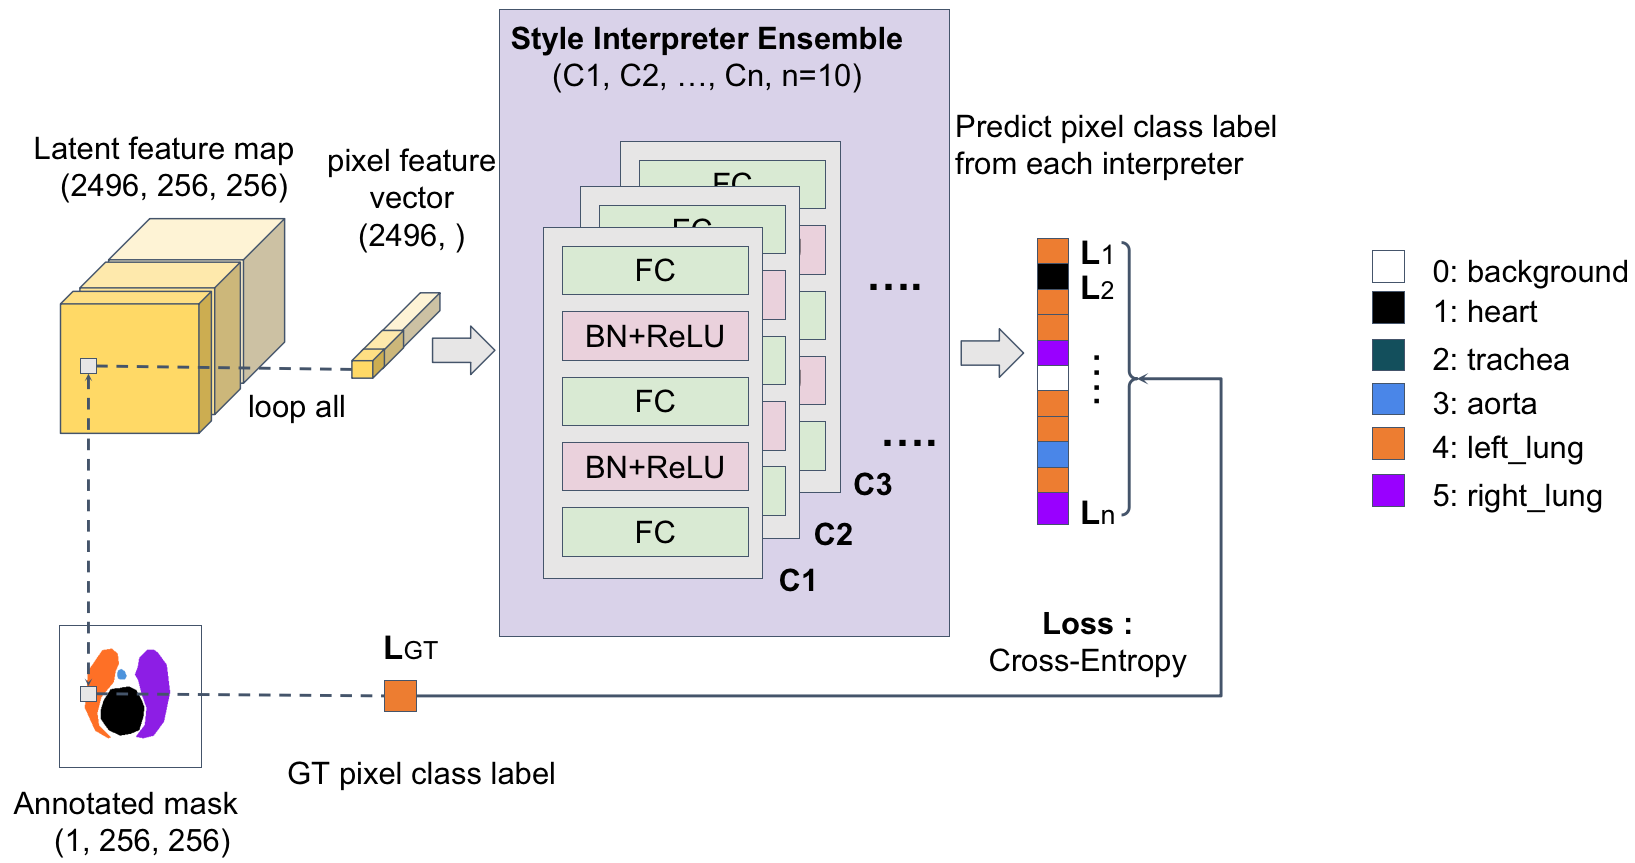
\includegraphics[width=0.75\textwidth]{./fig/style-interp.png}
  \caption{The style interpreter training framework. \textbf{BN}: batch normalization; \textbf{$P_{k}$} is the $k$th pixel classifier of the pixel classifier ensemble; \textbf{$C_{k}$} is the predicted class label of a given pixel by $k$th pixel classifier, while \textbf{$C_{GT}$} is the ground truth class label of the pixel.}
  \label{fig:interpreter}
\end{figure*}

\subsection{Revised DatasetGAN architecture for medical images}
\subsubsection{Replace StyleGAN2 for StyleGAN:}
Training a high-performance style-based generator is essential to generate high-quality images simulating the sought-after data distribution. 
Although StyleGAN used in original DatasetGAN can produce visually realistic images, the adaptive instance normalization (AdaIN) layer in StyleGAN style block may cause blob-like artifacts, plaguing the generated image quality.
Several improvements have been proposed to the StyleGAN architecture and training strategy in StyleGAN2~\cite{Karras2020AnalyzingAI}, including 1). the AdaIN layer in StyleGAN is broken to explicit normalization followed by modulation, as shown in Fig.~\ref{fig:stylegan2}; 2) the addition of bias and noise broadcast operation is moved to
be outside the active area of a style; 3) adjust only the standard deviation per feature map.
Previous studies have proved the effectiveness of these modifications in improving the generative performance in terms of commonly used evaluation metrics. 
More details about these improvements can be found in the StyleGAN2 paper~\cite{Karras2020AnalyzingAI}.

\begin{figure}[!ht]
  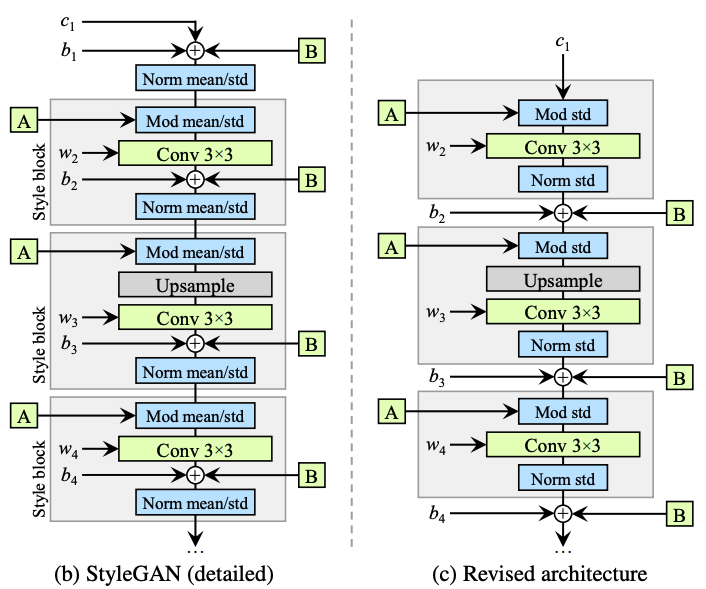
\includegraphics[width=0.5\textwidth]{./fig/stylegan2_blk.png} 
  \caption{The architecture of the style block in StyleGAN2. 
  Image credit: Karras \etal, 2020\cite{Karras2020AnalyzingAI}}
  \label{fig:stylegan2}
\end{figure}

\subsection{applying adaptive discriminator augmentation (ADA) strategy to training StyleGAN2} 
As Karras discussed in StyleGAN2 paper~\cite{Karras2020AnalyzingAI}, another limitation of StyleGAN is that Training a high-quality, high-resolution GAN generator usually needs $10^5-10^6$ images to avoid overfitting~\cite{karras2020training}. 
This is an even exaggerated challenge in medical imaging synthesis tasks, because large amounts of data are usually not available due to small sample population or confidential concerns. Using small datasets makes the discriminator trapped in an overfitting problem. 
For example, the original DatasetGAN used the NABirds dataset with 48k images to train StyleGAN without data augmentation~\cite{Zhang2021DatasetGANEL}. 
Although a few large medical image datasets are available, the broad applications of DatasetGAN to medical imaging requires that the style-based generator must learn from smaller datasets that are much more common and easier to collect in practical situations. 
To alleviate the overfitting problem on small datasets, ADA proposed by Karras et.al~\cite{karras2020training} is employed before the discriminator as data augmentation when training the style-based generator. 
As shown in Fig.~\ref{fig:ada}, it is an adaptive data augmentation (ADA) pipeline that tunes the augmentation strength dynamically based on the degree of overfitting, which enables training of the discriminator without leaking the augmentation pattern. 
The experiment results indicate that ADA could significantly improve the performance of the style-based generator on small datasets~\cite{karras2020training}.  

\begin{figure}[!ht]
  \centering
  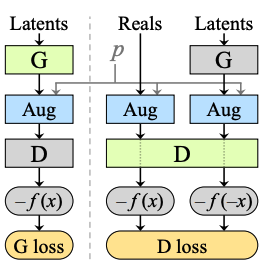
\includegraphics[width=0.3\textwidth]{./fig/ada.png} 
  \caption{Flow chart of stochastic discriminator augmentation. The blue elements highlight operations related to augmentations, while the rest implement standard GAN training with generator G and discriminator D.
  Image credit: Karras \etal, 2020\cite{karras2020training}}
  \label{fig:ada}
\end{figure}

\subsection{Datasets and implementation details}
\label{sec:impl}
\noindent \textbf{Datasets}:
In this study, we employed SegTHOR dataset~\cite{Lambert2020SegTHORSO} to train the StyleGAN2 generator. SegTHOR dataset is a Computed Tomography (CT) dataset with image size of $512\times 512$ pixels from 60 patients with non-small cell lung cancer. 
These images were segmented with 5 kinds of organ masks: heart, aorta, trachea, left-lung and right-lung. 
We select 2377 annotated slices that have lungs as the training dataset to train the StyleGAN2 generator. We suppose images with lungs share lower intra-class variance compared to other body sections, thus improving the image generation quality when dealing with limited training data. Fig.~\ref{fig:real_data} shows several examples of the selected CT slices. 

\begin{figure}[h]
    \centering
    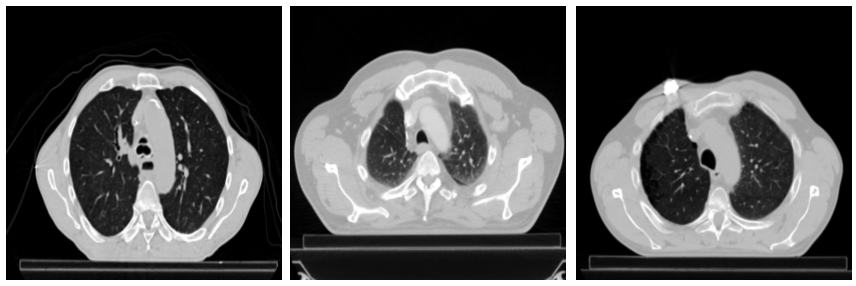
\includegraphics[width=0.5\textwidth]{./fig/real_sample.png}
    \caption{Examples of training SegTHOR CT slices.}
    \label{fig:real_data}
\end{figure}

\noindent \textbf{Training StyleGAN2}:
\label{sec:train_gan}
We adapt the official stylegan2-ada-pytorch repository to train the StyleGAN2 generator (\url{https://github.com/NVlabs/stylegan2-ada-pytorch.git}). The training process is shown in Fig.~\ref{fig:stylegan2}. The network architecture is described as section~\ref{sec:stylegan}, while the training techniques include enabling ADA augmentation strategy and setting $R_1$ regularization weight $\gamma$ as 1. Keep other parameters default. The SegTHOR training images are preprocessed by center-cropping and resizing to a fixed image size as $256\times 256$ pixels. The training process ends after learning $10^7$ batches of real images. 

\noindent \textbf{Training style interpreter}
The style interpreter's inputs are the latent features produced by StyleGAN2 by feeding the random vector $z$. In another word, the training input data of the style interpreter is synthesized rather than real. Therefore, to train the pixel classifier, we manually segment 30 generated images corresponding to the latent features as the ground-truth (GT) segmentation data. 
In this study, the segmented organs include additional left lung, and right lung, roughly balancing the number of pixels belonging to the background class and other organ classes to improve training stability. 
Note each latent feature map and corresponding segmentation mask are flattened to generate 65536 4992-dimensional pixel vectors and 65536 pixel labels. So all the 30 latent feature maps and annotated masks are processed using this method to make a training dataset for pixel classifier, with total of 1966080 pairs of pixel vector and GT class label. 

The network architecture and training process are shown in Fig.~\ref{fig:interpreter}. For the 10 pixel classifiers in the ensemble, we iteratively train the classifier on the same training dataset while the parameters of each network are initialized with Kaiming initialization strategy~\cite{He2015DelvingDI}. The network is trained with cross-entropy loss for 100 epochs and Adam stochastic gradient algorithm~\cite{Kingma2015AdamAM} is employed to perform the optimization of model parameters. The initial learning rate is set to 0.0001

\vspace{-0.2cm}
\section{Results}
\subsection{DatasetGAN generated data}.
\label{sec:generated_data}
Fig.~\ref{fig:generated_data} shows samples of DatasetGAN generated image and segmentation mask pairs. We notice that some annotations have misclassified pixels, perhaps due to the failure of StyleGAN2 generator or the pixel classifier ensemble. 
According to the percentage of misclassified pixels, the generated image-mask pairs could be divided into 3 categories: good, partial-bad, and bad case. The good case roughly has $\le 1\%$ incorrect labels. 
The bad case has $\ge 25\%$ incorrect labels, and the partial-bad is in between. 
We analyzed 100 random DatasetGAN generated image-mask pairs and categorized them in this rule. The ratio between good/bad/partial-bad is 74/15/11, validating that the StyleGAN2 might introduce noise in the synthesized dataset. 
To reduce the uncertainties in the generated data, improving the performance of the style-based generator seems to be the critical step. 

\subsection{Effect of the proposed revisions to the performance of DatasetGAN}
\label{sec:abl_datasetgan}
With these two revisions during training StyleGAN2-based generator, the Frechet inception distance (FID) score of the synthetic images of the StyleGAN2 generator improved to $43.02$, while the FID of generated images using the original DatasetGAN architecture only reached $56.34$.
However, the analysis results discussed in previous sections imply that the generator still had limited performance in synthesizing datasets which deviated from the distribution of real data. More techniques would be investigated to improve the training of StyleGAN2 generator.

\begin{figure*}[h]
  \centering
  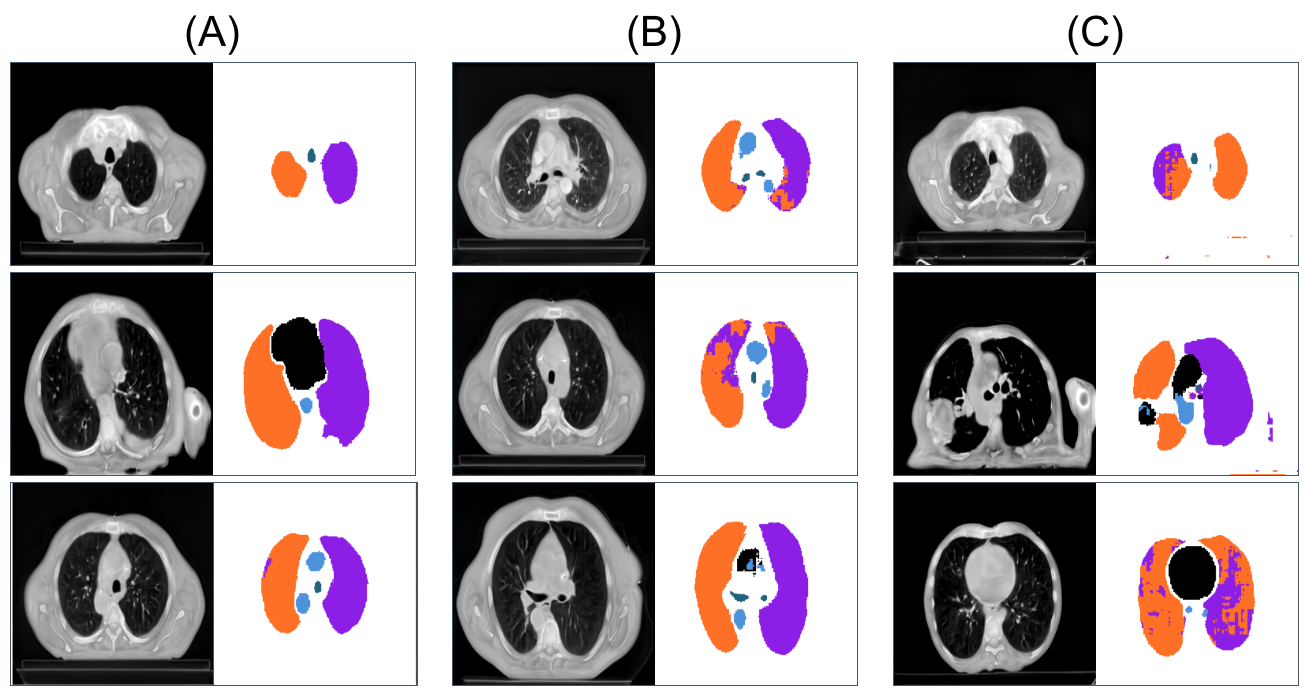
\includegraphics[width=0.9\textwidth]{./fig/generated_sample.png}
  \caption{Examples of DatasetGAN generated images and segmentation masks. \textbf{A}: good case; \textbf{B}: partial-bad case; \textbf{C}: bad case.}
  \label{fig:generated_data}
\end{figure*}

\subsection{DatasetGAN evaluation on parts segmentation}
\label{sec:eval}
Intuitively, if the DatasetGAN generated images and masks are convincing enough, 
a segmentation network trained on the synthetic dataset should have similar performance compared to being trained on the real dataset. 
The performance of the trained segmentation network seems to be positively related to the quality of DatasetGAN generated data. 
We evaluated the quality of DatasetGAN generated image-mask pairs via part segmentation. DeepLab-V3-ResNet101~\cite{chen2017rethinking} was employed as the segmentation network trained on both DatasetGAN generated datasets. 
The training dataset contained 1500 synthetic image-mask pairs. The trained networks were evaluated using 5 cross-fold validation on both generated testing dataset (test-G) and real-image testing dataset (test-R), respectively. 
They contained another 100 generated or real human-labeled image-mask pairs. Mean intersection over union (mIoU) and standard deviation were calculated as the metrics of segmentation performance. 

The trained DeepLab-V3 achieved mIoU as $0.773\pm 0.012$ on test-G and $0.551\pm 0.006$ on test-R, indicating that there was an obvious distribution gap between the generated image and real image. For further comparison, we trained the segmentation network on pure real training dataset with 500 human-labeled SegTHOR image-mask pairs. Similarly, the performance gap existed: the mIoU testing result was $0.459\pm 0.004$ on test-G and $0.799\pm 0.010$ on test-R. 
We suppose adding a few real data to the generated training data may narrow the gap when training the segmentation network. A hybrid training dataset was made to train the segmentation network, which combined 1500 generated synthetic image-mask pairs with 30 real SegTHOR image-mask pairs. The performance gap on test-G and test-R were filled, achieving $0.775\pm 0.012$ and $0.762\pm 0.006$, respectively. 
The result demonstrates that adding few real data does benefit the training of segmentation network by preventing overfitting to the intrinsic noise of generated data, especially when the quality of the trained style-based generator is suboptimal. 

\subsection{Analysis of segmentation performance-related factors}
\subsubsection{Synthesized segmentation dataset size} 
As shown in table~\ref{table:abl_seg}, we increased the number of generated segmentation training images from 1500 to 15000 image-mask pairs. As the number of images increased, the segmentation performance was also improved. 

\begin{table}[!h]
  \centering
  \begin{tabular}{c||c|c}
    \hline 
     & mIoU on test-G & mIoU on test-R  \\
    \hline
    Dataset size=1.5k & $0.773\pm 0.012$ & $0.551\pm 0.006$ \\
    Dataset size=5k & $0.783\pm 0.011$ & $0.560\pm 0.010$ \\
    Dataset size=10k & $0.793\pm 0.010$ & $0.569\pm 0.007$ \\
    Dataset size=15k & $\mathbf{0.801\pm 0.009}$ & $\mathbf{0.580\pm 0.007}$ \\
    \hline
  \end{tabular}
  \vspace{0.05cm}
  \captionof{table}{The synthesized segmentation training dataset size vs mIoU.}
  \label{table:abl_seg}
\end{table}

\subsubsection{Annoated style-interpreter dataset size}
In principle, a larger dataset for training style-interpreter is better since such dataset is more representative of real image data distribution. A better style interpreter corresponds to higher synthetic segmentation quality. 
We trained the pixel classifier ensemble with $k=30, 50, 100$ human-labeled image-mask pairs. Then the trained DatasetGAN-StyleGAN2s generated the synthetic segmentation dataset for further parts segmentation described in section~\ref{sec:eval}. As shown in table~\ref{table:abl_dataset}, using more labeled data could improve the performance of pixel classifiers significantly. It implies that expanding the human-labeled samples could leverage the performance of DatasetGAN-StyleGAN2 even when the performance of the style-based generator is limited. 

\begin{table}[!h]
  \centering
  \begin{tabular}{c||c|c}
    \hline 
     & mIoU on test-G & mIoU on test-R  \\
    \hline
    Annotated images=30 & $0.773\pm 0.012$ & $0.551\pm 0.006$ \\
    Annotated images=50 & $0.798\pm 0.004$ & $0.626\pm 0.004$ \\
    Annotated images=100 & $\mathbf{0.844\pm 0.005}$ & $\mathbf{0.663\pm 0.004}$ \\
    \hline
  \end{tabular}
  \vspace{0.05cm}
  \captionof{table}{Manually-annotated style-intepreter dataset size vs mIoU.}
  \label{table:abl_dataset}
\end{table}  

\section{Discussion}
This study investigated the potential applications of DatasetGAN in medical imaging.
The experimental results indicated that DatasetGAN can be employed to provide reliable segmented medical images to support clinical practice. 
Our revisions on the style-based generator are effective to tailor DatasetGAN for small datasets. 
In addition, the effectiveness of the framework was evaluated from multiple perspectives.
The performance of our DatasetGAN-R was evaluated both with qualitative and quantitative metrics.  
Factors such as training dataset size and latent selection strategy which may have impacts on the performance of DatasetGAN-R were also investigated.
Overall, this work shows that a well-trained DatasetGAN could synthesize massive high-quality segmentation datasets, holding the potential for multiple medical applications.

A well-trained DatasetGAN works as a powerful automatic labeling factory, which could easily produce a large dataset with both realistic images and corresponding high-quality segmentation data. As we discussed in previous sections, the performance of the segmentation network trained on the synthetic dataset positively reflects the performance when trained on the real dataset. 
One interesting potential application of DatasetGAN is that it works as a standard dataset generator for an objective evaluation of segmentation methods. 
In this way, manual annotation bias is minimized in the generated dataset. Different methods proposed by researchers could be trained and objectively evaluated using the dataset. 
For example, if we aim to find a potential optimal segmentation method on SegTHOR dataset. 
Another two widely-used segmentation networks, FCN~\cite{long2015fully} and UNet~\cite{Ronneberger2015UNetCN}, can be exploited while the DeepLab-V3 is treated as the baseline. 
Performance evaluation is shown table~\ref{table:diff_networks}. The results demonstrate the FCN is probably the most suitable method for SegTHOR dataset. 
In the future, further studies should be conducted to improve the quality of synthesized images (e.g., the accuracy of masks) to warrant its potential to support clinical practice.

\begin{table}[h!]
  \centering
  \begin{tabular}{c||c|c|c}
    \hline 
     & \textbf{Deeplab-V3} & \textbf{FCN} & \textbf{UNet} \\
    \hline
    mIoU on test-G & $0.773\pm 0.012$ & $\mathbf{0.798\pm 0.014}$ & $0.782\pm 0.013$ \\
    mIoU on test-R &  $0.551\pm 0.006$ & $\mathbf{0.589\pm 0.004}$ & $0.566\pm 0.009$  \\
    \hline
  \end{tabular}
  \vspace{0.05cm}
  \captionof{table}{Objective evaluation of different segmentation networks.}
  \label{table:diff_networks}
\end{table} 


\vspace{-0.2cm}
\scriptsize{
\bibliographystyle{IEEEtran}
\bibliography{ref}
}

\end{document} 